\documentclass[conference]{IEEEtran}
\IEEEoverridecommandlockouts
% The preceding line is only needed to identify funding in the first footnote. If that is unneeded, please comment it out.
\usepackage{cite}
\usepackage{amsmath,amssymb,amsfonts}
\usepackage{algorithmic}
\usepackage{graphicx}
\usepackage{textcomp}
\usepackage{xcolor}
\usepackage{verbatim}
\usepackage{footnote}
\usepackage{xr}

\def\BibTeX{{\rm B\kern-.05em{\sc i\kern-.025em b}\kern-.08em
    T\kern-.1667em\lower.7ex\hbox{E}\kern-.125emX}}


\newtheorem{constraint}{\textbf{Constraint}}

\newenvironment{defn}
{\vspace{12pt} \noindent {\textit{meaning:}}} \\

\begin{document}

\title{Paper Title*\\
{\footnotesize \textsuperscript{*}Note: Sub-titles are not captured in Xplore and
should not be used}
\thanks{Identify applicable funding agency here. If none, delete this.}
}

\author{\IEEEauthorblockN{1\textsuperscript{st} Given Name Surname}
\IEEEauthorblockA{\textit{dept. name of organization (of Aff.)} \\
\textit{name of organization (of Aff.)}\\
City, Country \\
email address}
\and
\IEEEauthorblockN{2\textsuperscript{nd} Given Name Surname}
\IEEEauthorblockA{\textit{dept. name of organization (of Aff.)} \\
\textit{name of organization (of Aff.)}\\
City, Country \\
email address}
}

\maketitle

\begin{abstract}
Floorplanning is a mandatory step in the design of hardware accelerators on FPGA platforms consisting in placing the hardware modules to specific FPGA areas. In particular, if the design makes use of partial reconfiguration (PR), the overall system performance is greatly influenced by the allocation strategy. Existing tools for PR, which are provided by FPGA vendors, allow floorplanning to be performed manually. This method besides being highly time-consuming, demands a good knowledge of the architecture and organization of the hardware for an optimal floorplan. To solve this problem, this paper presents an automated floorplanner based on Mixed Integer Programming (MILP). The most common approach by the state of the art automated MILP (or other optimization method) based floorplanners is to apply MILP (or other optimization methods) for finding the optimal placement from a pre-enumerated list of possible placements. Meanwhile, in this work, the floorplanning problem was directly solved as an optimization problem by modeling the FPGA resources as a set of MILP constraints along with the standard PR related constraints. The performance of the proposed approach was tested by using a synthethic benchmark suite. Its performance was also compared with the state of the art MILP based floorplanners for the average execution time. Finally, the floorplanner was used in a real case study. This approach was observed to improve the execution time reported in the state of the art by orders of magnitude.
\end{abstract}

\begin{IEEEkeywords}
component, formatting, style, styling, insert
\end{IEEEkeywords}

\section{Introduction}
\textbf{par 1} \\
\textit{what is floorplanning and how is it applied (what's its role) in the context of PR, what is the benefit of having a good floorplan or a floorplan at all} \\

\textbf{par 2} \\
\textit{How is fp done currently and what are the shortcomings of those methods} \\

\textbf{par 3} \\
\textit{In short what did I do and what are my contributions (clearly stated)} \\

\textbf{par 4} \\
\textit{organization of the paper} \\

Floorplanning is one of the major challenges in the field of dynamic parital reconfiguration. The placement of the static and reconfigurable slots on the FPGA fabric must satisfy the application requirements set by the application designer while also respecting the technological constraints set by the manufacturer. The conventional approach for an automated generation of FPGA floorplans usually involves two steps. First for each slot, all the possible rectangular slots that satisfy the resources requirement of the slot are enumerated. This is done by starting a scan on the fpga fabric from the bottom left corner and lisitng all the rectangles that contain all the necessary resources for the respective slots. Then some sort of heuristics/optimization is applied to choose the optimal ones from the set of possible slots. This approach has many problems \{\textit{to be listed later}\}\\\\

Our approach instead focuses on applying the optimization process on a lower level of abstraction of the fpga fabric i.e., rather than applying optimization to select the most optimal one from a set of pre-scanned slots, we modeled the different types of resources on the fpga and their distribution along with forbidden regions as a set of constraints and added these constraints to the predefined constraints related to dpr. \\

Let us consider a floorplanning example where we have to make a floorplan for two slots S$_1$ and S$_2$ on the FPGA fabric. Each slot has resource requirements denoted as \{D$_1$, B$_1$, C$_1$\} and \{D$_2$, B$_2$, C$_2$\} where D, B and C represent DSP, BRAM and CLB respectively. \\ Our proposed system takes as an input in the resource requirement of each slot and a description of the resource distribution of the FPGA fabric and it returns the placement coordinates of the slots on the fpga fabric. \\
A slot is represented using 4 parameters i.e. the two bottom left coordinates and the width and the height of the slot. In our considered example the slots S$_1$ and S$_2$ are represented as (x$_1$, y$_1$, w$_1$, h$_1$) and (x$_2$, y$_2$, w$_2$, h$_2$). A forbidden region is also represented as a slot hence a forbidden region F$_i$ can be represented as {fx$_i$, fy$_k$, fw$_i$, fy$_i$}  \\ 



\section{Related Works}
\section{Background and Modeling}
In this section we breifly describe the general architecture of FPGAs, the design flow in partial reconfiguration (PR) and the assumptions that led to the fromulation of PR floorplanning problem as a MILP problem. This work is based on the 7 series FPGA family from Xilinx. \\

\subsection{FPGA Architecture and Partial-Reconfiguration}

The configurable fabric of Xilinx FPGAs is divided into quadrants named clock regions. Within each clock region there are columns of different configurable resources such as CLBs, BRAMs or DSPs.  Resources within a clock region share the same clock. A single column in a clock region is referred to as a tile. The number of resources in a tile varies depending on the device family. For example in Virtex 7z a CLB tile contains 50 clbs a BRAM tile contains 10 brams and a DSP tile contains 20 dsps. The functional logic compoenets (clbs, brams and dsps) and the routing logic components (switches, interconnects etc...) on the FPGA are configured based on a bit file stored in the configuration memory of an FPGA. This memory is organized into minimal configurable units called frames. A single frame in the configuration memory corresponds to a single tile on the fabric. In addition to the above mentioned resources, FPGAs also contain other components such as clock and clock modifying logic, I/O logic, configuration logic etc... Depending on the type of device family some of these components may or may not be included in a reconfigurable region. FPGAs, in particular 7 series devices, which are subject of this work, also contian routing resources called interconnect tiles. These tiles are placed back-to-back as shown in Fig \ref{fig:fpga}. When floorplanning for partial reconfiguration, the position of these back-to-back boundaries must be known inorder not to split them and violate PR restriction.

\begin{figure}
  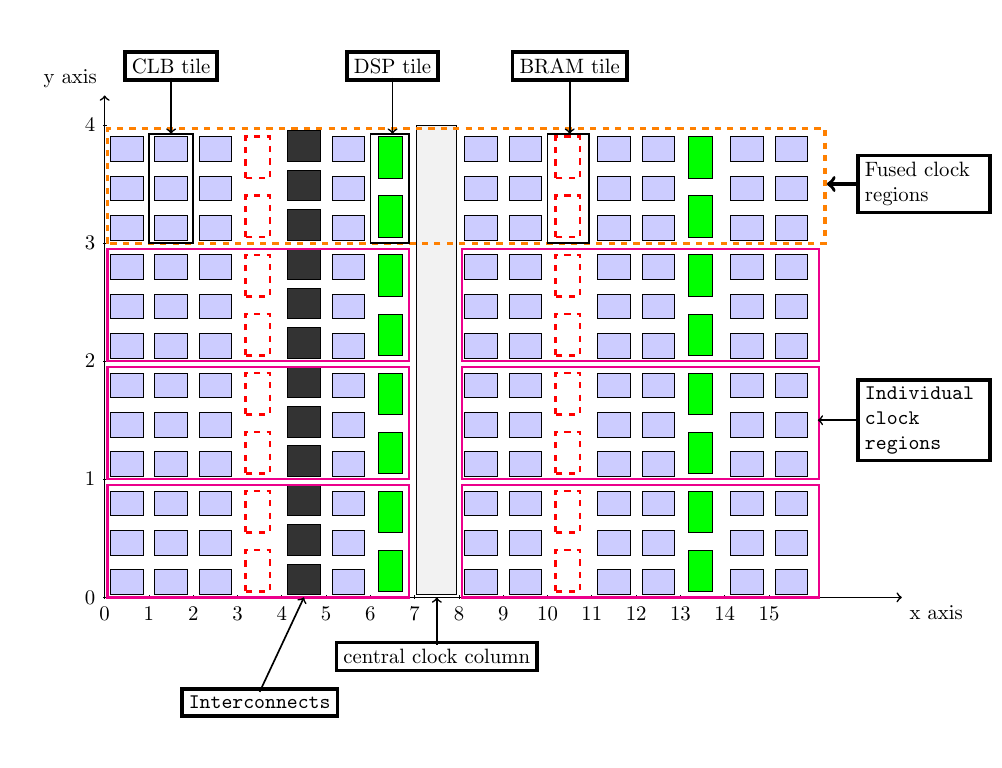
\includegraphics[width=\linewidth]{graphics/fpga.png}
  \caption{FPGA architecture}
  \label{fig:fpga}
\end{figure}

Partially reconfigurable applications are often composed of \textbf{\textit{M$_s$}} number of static and \textbf{\textit{M$_r$}} number of reconfigurable modules that are to be placed in \textbf{N$_s$} static and \textbf{N$_r$} reconfigurable regions on the FPGA respectively.  In PR applications the number of static modules equals to the number of static regions i.e., \textit{M$_s$ = N$_s$} while the number of reconfigurable modules is always greater than reconfigurable regions i.e., \textit{M$_r$ $>$ N$_r$}. Floorplanning in PR can then be defined as the process of allocating placement for \textit{N$_r$} reconfigurable regions on the FPGA fabric. \\

\textbf{state how PR-fp is currently done in vivado} \\

\subsection{Combining clock regions}
On Xilinx FPGAs, the central clock column divides the FPGA into left and right regions as shown on fig \ref{fig:fpga}. But in our model all the horizontally adjacent clock regions were fused into a single clock region. This simplifies our modeling with no penalty. As also shown in the figure on fig \ref{fig:fpga}, a cartesian coordinate system can be overlayed on FPGAs to uniquely identify each resource on the logic fabric. The x axis represents each column of resources while the rows on the y axis represent the fused horizontally adjacent clock regions as indicated on fig \ref{fig:fpga}. Combining the horizontally adjacent clock regions\footnote{henceforth clock regions implies horizontally fused clock regions}, in addition to resulting in a lower range of variables on the y axis, organizes resources on the y axis on a per tile (per clock region) basis instead of as individual clbs, brams or dsps. This reduces the search space for the solution in the MILP formulation at the expense of wasting resources. Based on this abstraction the resources on the FPGA fabric on a tile basis, the FPGA would become \textbf{W} columns wide and \textbf{H} clock regions high.  \\

The i\textsuperscript{th} reconfigurable region R$_i$ is a rectangular region on the FPGA fabric that hosts, at different durations, the set of reconfigurable modules assigned to it. R$_i$ can be represented as
\begin{equation}
R_i = (x_i, y_i, w_i, h_i) \mid x_i + w_i \leq W, y_i + h_i \leq H
\end{equation}

where x$_i$ and y$_i$ represent the bottom left coordinate and w$_i$ and h$_i$ represent the width and height of R$_i$ resectively. A resource type \textit{t} that is required by reconfigurable module \textit{M$_r$} is denoted as \textit{c$_{rt}$} while the same type of resource that is incorporated inside a reconfigurable region R$_i$ is denoted as $\eta_{it}$. The upper and lower boundaries of R$_i$ are aligned to clock region boundaries since the resources on the fabric are organized on a tile basis. 

\textbf{\\talk about the modeling of forbidden regions}

\subsection{Discretization of the axis}
Floorplanning is a two dimensional (quadratic) problem in that determining the number of resource contained in R$_i$ invloves determining the resources on both axis i.e., the area of the rectangle. To linearize this problem either of the axis must be discretized. A good strategy for discretization would be choosing the axis with the lower range of variables as this leads to an easily scalable model. In all the FPGA families that were chosen to be studied for this project, the range of the y axis (the number of clock regions on the y axis) was less than the range of the x axis i.e., H $<$ W. For example in kintex xc7z045fbv676 there are 100 columns on the x axis as opposed to 7 clock regions on the y axis. Hence the binary variable $\beta_{ij}$ denotes clock region j in region in R$_i$. \\

%$\forall$ i = 1...,N$_r$,  $\forall$ j = 1...,H \\
%$\beta_{ij}$ $\in$ [0,1] $\mid$ $\beta_{ij}$ represents clock region j in R$_i$. \\

\subsection{FPGA resource finger-printing} 
Resources in most Xilinx FPGAs are distributed in a redundant manner this is to say vertically adjacent clock regions have a fairly similar distribution of resources with the possibility of different forbidden regions being included in them. Hence the reconfigurable fabric of most Xilinx FPGAs can accurately be represented by describing the resources in a single clock region and the location of forbidden regions in all clock regions. This process is equivalent to developing the resource distribution finger-print of a specifc type of FPGA. For each resource type \textit{t} a piecewise function f$_t$(x) can be used to describe the distribution of that particular resource inside the first clock region of the FPGA along the x axis. As an example f$_t$(x) for the first clock region on fig \ref{fig:fpga} would be 

\begin{figure}
  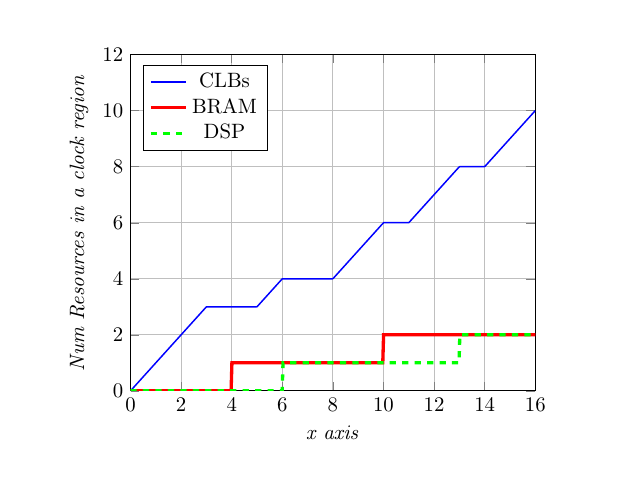
\includegraphics[width=\linewidth]{graphics/resource.png}
  \caption{Resource distribution finger print of fig \ref{fig:fpga}}
  \label{fig:finger-print}
\end{figure}


\begin{comment}
\begin{equation}
f_c(x) = \begin{cases}
\mu_c * x, & \textbf{ 0$\leq$x$<$4}, \\
\mu_c * (x-1), & \textbf{4$\leq$x$<$7}, \\
\mu_c * (x-2), & \textbf{7$\leq$x$<$W}, \\
\end{cases}
\end{equation}
\end{comment}

%\textbf{fig} depicts f$_t$(x) for the first clock region zynq xc7z015.

If $\mu_t$ is a constant that denotes the number of resource \textit{t} per tile, the amount of each type of resource included inside a region R$_i$ i.e., $\eta_it$ can be defined as \\

\begin{equation}
\label{model:eq:4}
\eta_{it} = \sum_{j=1}^{H} \beta_{ij} \cdot (f_t(x_i+w_i) - f_t(x_i)) * \mu_t
\end{equation}

\begin{comment}
The set of components that must not be included in 
A reconfigurable region R$_i$ must, at the very least, incorporate the resources required by the largest reconfigurable module that it hosts. Reconfigurable regions are rectangular in shape and to ease the routing during implementation, the height of the reconfigurable region must be aligned to clock region boundaries.\\
\end{comment}

\section{Floorplanning problem formulation}

\textbf{\\ put a picture of PR design flow in Xilinx} \\

Partial-reconfiguration involves dynamically switching modules in a reconfigurable region whilst other reconfigurable and static regions continue to be operational. \textbf{Fig} depicts the PR design flow in Xilinx FPGAs as implemented in Xilinx Vivado. The major steps in the automated PR flow are \\

\begin{itemize}
\item \textit{Synthesis}: At this level the behavioral description of modules written in hardware description langauges (Verilog or VHDL) is converted into a gate-level netlist. In PR design flow, floorplanning is mandatory (it is optional in the standard flow) and it must be done before the implementation step.  
\item \textit{Implementation}: In this step the gate-level netlist output of the previous stage is functionally mapped to specific device resources on the FPGA and then placed and routed.
\item \textit{Bitstream generation}: In PR desgin flow, the final output of an FPGA design tool is a set of bit files which contain the configuration information for both the logic and routing resources of the static and reconfigurable regions. 
\end{itemize} 

\hfill \break

In floorplanning for PR, each R$_i$, which are also named \textit{Pblocks} in the Xilinx design flow, are subject to the following restrictions and requirements. 

\begin{enumerate}
\item Reconfigurable regions must contain only valid reconfigurable resources (for example in 7 series FPGAs only CLBs, BRAMs and DSPs must be in R$_i$)
\item The minimum number of resources incorporated by a reconfigurable region \textbf{R$_i$} (Pblock) must at least be equal to the resource requirement of the largest module hosted in the region

\item Two reconfigurable regions must not overlap. Overlapping is equivalent to sharing at least a single tile

\item The left and right edges of R$_i$ must not split interconnect columns 

\item Reconfigurable regions(Pblocks) can span non reconfigurable components such as configuration blocks, central clock column etc... without considering them as part of the region(Pblocks)

\item The height of R$_i$ must be aligned to clock regions. This is an optional requirement but enforcing it results in starting the reconfigurable module from a known initial state re-configuration

\end{enumerate}



\begin{comment}
The central clock column divides the FPGA into left and right regions as shown in the figure. But all the horizontally adjacent clock regions are combined into a single clock region to make the x axis W units wide. The y axis is H units high. Combining horizontally adjacent clock regions into a single clock region does

Reconfigurable regions need not necessarily be rectangular but assigning rectangular shapes to regions greatly reduces routing and placement challenges

The bit files are deployed in the FPGA configuration memory. 
\end{comment}
\section{MILP formulation}
In this section the MILP model of the PR floorplanning problem is presented. The section first summarizes the considered assumptions and abstractions related both to the FPGA and its resources as well as the floorplanning problem. The description of the model consists of defining variables, constraints and an objective function to be optimized. 

% also add how the central clock column is modeled as a forbidden region}. \\

%The total number of a resource R within a slot S$_i$ = (x$_i$, y$_i$, w$_i$, h$_i$) is then equal to
%\begin{equation}
%R = (x_i + w_i) \cdot (y_i + h_i)
%\end{equation}  



\subsection{definition of optimization variables}
\begin{comment}
To encode the MILP formulation the following binary and real variables are defined. \\ \\
Variables related to the size, location and number of resources in slot S$_i$. \\
For each slot S$_i$
\begin{itemize}
\item N: set of reconfigurable regions

\item S$_i$: slot i $\mid$ S$_i$ $\in$ N 

\item W $\in$ $\mathbb{Z}$ represents the total width of the fpga fabric

\item H $\in$ $\mathbb{Z}$ specifies the height of the fpga fabric

\item C: the set of clock regions on the fpga

\item r $\in$ $\mathbb{Z}$ denotes the number of rows inside a single clock region

\item F: set of forbidden regions

\item F$_k$: forbidden region k $\in$ F

\item x$_i$, y$_i$ w$_i$, h$_i$ $\in$ $\mathbb{Z}$ represent the bottom left coordinates, the width and the height of S$_i$  respectively
\end{itemize}

\begin{itemize}
\item clb$_i$, bram$_i$ and dsp$_i$  $\in$ $\mathbb{Z}$ represent the number of clb, bram and dsp between x$_i$ and x$_i$ + w$_i$ in a single row respectively.
\end{itemize}

\begin{itemize}
\item clb$\_$req$_i$, bram$\_$req$_i$ and dsp$\_$req$_i$ $\in$ $\mathbb{Z}$ represent the required number of clb, bram and dsp in S$_i$.
\end{itemize}

\begin{itemize}
\item $\beta_{ijk}$ $\in$ [0,1] represents row k in clock region j for slot S$_i$.
\end{itemize}

\end{comment}

\hfill \break
Variables denoting the relationship between two slots 

For two slots S$_i$ and S$_k$ 
\begin{itemize}
\item $\gamma_{ik}$ $\in$ [0,1] is a binary variable used to identify whether S$_i$ is found on the left or on the right of S$_k$\\
$\gamma_{ik}$ = 1 if x$_i$ $\leq$ x$_k$ [i.e. S$_i$ is on the left of S$_k$]

\begin{comment}
\item $\theta_{ik}$ $\in$ [0,1] is a binary variable used to identify whether S$_i$ is found on the top or bottom of of S$_k$\\
$\theta_{ik}$ = 1 if y$_i$ $\leq$ y$_k$ [i.e. S$_i$ is found below S$_k$]

\item $\Gamma_{ik}$ $\in$ [0,1] is used to denote if bottom right x coordinate of S$_i$ is found to the right of the bottom left coordinate of S$_k$ \\
$\Gamma$ = 1 if x$_i$ + w$_i$ $\geq$ x$_k$

\item $\eta_{ik}$ $\in$ [0,1] is used to denote if bottom right x coordinate of S$_k$ is found to the right of the bottom left coordinate of S$_i$ \\
$\eta$ = 1 if x$_k$ + w$_k$ $\geq$ x$_i$

\item $\Omega_{ik}$ $\in$ [0,1] is used to denote if the top y coordinate of S$_i$ is found above the lower y coordinate of S$_k$ \\
$\Omega$ = 1 if y$_i$ + h$_i$ $\geq$ y$_k$

\item $\Psi_{ik}$ $\in$ [0,1] is used to denote if top y coordinate of S$_k$ is found above the lower y coordinate of S$_i$ \\
$\Psi$ = 1 if y$_k$ + h$_k$ $\geq$ y$_i$


\item $\Delta_{ik}$ $\in$ [0,1] is a binary variable which indicates interfernce between slots S$_i$ and S$_k$.\\
$\Delta_{ik}$ = 0 if there is no interference between the slots [i.e. not a single tile is shared between slots]

\end{comment}
%\item D$_{w}$, B$_w$ and C$_w$ represent wasted DSPs, BRAMs and CLBs in S$_i$ respectively
%\item $\alpha_i$ is a real variable that is used to express the bound on the amount of wasted resources in a slot S$_i$
%\item $\rho$ and $\nu$ are vectors which contain the x and y coordinates of all the forbidden columns and rows on the FPGA fabric respectively 
%\item $\eta_{ik}$ is a real variable that expresses the bound on the wirelength between S$_i$ and S$_k$
\end{itemize}

\hfill \break

\begin{comment}
Variables denoting the relationship between S$_i$ and forbidden region F$_k$.  
\begin{itemize}
\item $\mu_{ik}$ $\in$ [0,1] is a binary variable used to identify whether S$_i$ is found on the left or on the right of F$_k$\\
$\mu_{ik}$ = 1 if x$_i$ $\leq$ fx$_k$ [i.e. S$_i$ is on the left of F$_k$]

\item $\nu_{ik}$ $\in$ [0,1] is a binary variable used to identify whether S$_i$ is found on the top or bottom of of F$_k$\\
$\nu_{ik}$ = 1 if y$_i$ $\leq$ fy$_k$ [i.e. S$_i$ is found below F$_k$]

\item fbdn$_1$ $\in$ [0,1] is used to denote if bottom right x coordinate of S$_i$ is found to the right of the bottom left coordinate of F$_k$ \\
fbdn$_1$ = 1 if x$_i$ + w$_i$ $\geq$ fx$_k$

\item fbdn$_2$ $\in$ [0,1] is used to denote if bottom right x coordinate of F$_k$ is found to the right of the bottom left coordinate of s$_i$ \\
fbdn$_2$ = 1 if fx$_k$ + fw$_k$ $\geq$ x$_i$

\item fbdn$_3$ $\in$ [0,1] is used to denote if the top y coordinate of S$_i$ is found above the lower y coordinate of F$_k$ \\
fbdn$_3$ = 1 if y$_i$ + h$_i$ $\geq$ fy$_k$

\item fbdn$_4$ $\in$ [0,1] is used to denote if top y coordinate of F$_k$ is found above the lower y coordinate of S$_i$ \\
fbdn$\_4$ = 1 if fy$_k$ + fh$_k$ $\geq$ y$_i$
\end{itemize}

\hfill \break
\end{comment}
\subsection{Constraint definition}

\begin{comment}
Slots for partial reconfiguration should fulfill the following constraints
\begin{itemize}
\item there must be enough resources within the slots
\item A frame can not be shared between two reconfigurable partitions (no interference)
\item static resources on the FPGA must not be included in the slots 
\item Left and right edges of slots must be placed in proper positions
\item the amount of wasted resources should be minimized (Wasting DSPs is more expensive than BRAMs which in turn is more expensive than CLBs)
\item Other optimizations such as lower wire length between slots or lower length to I/O etc... can be added as constraints
\end{itemize}

\end{comment}
\hfill \break

\subsubsection{\textbf {Semantics constraints}}
The following constraints ensure the soundness of some of the variables.\\
\begin{constraint} $\forall$ S$_1$ $\in$ N, $\forall$ i = 1...,N\textsuperscript{max} , $\forall$ x$_i$ = 0..., W, $\forall$ y$_i$ = 0..., H $\forall$ w$_i$, $\forall$ h$_i$    
\begin{equation}
\begin{split}
x_i + w_i \leq W \\
y_i + h_i \leq H \\
\end{split}
\end{equation} 
\end{constraint}
\begin{defn} the right most x coordinate and the top y coordinates of S$_i$ must not exceed the boundaries of the fabric \\
\end{defn}

\begin{constraint} $\forall$ i = 1...,N\textsuperscript{max}, $\forall$ j = 1...,clk$\_$reg\textsuperscript{max}, $\forall$ k = 1...,r $\forall$ h$_i$
\begin{equation}
\begin{split}
 h_i = \sum_{j=1}^{clk\_reg} \sum_{k=1}^{r} \beta_{ijk}
\end{split}
\end{equation}
\end{constraint}

\begin{defn}
The height of S$_i$ must be the sum of binary rows in each clock region which are set to 1
\end{defn}

\begin{constraint} $\forall$ i = 1...,N\textsuperscript{max}, $\forall$ j = 1...,clk$\_$reg\textsuperscript{max}, $\forall$ k = 1...,r $\forall$ h$_i$
\begin{equation}
\begin{split}
y_i \leq \sum_{j=1}^{clk\_reg} \sum_{k=1}^{r} H - \beta_{ijk} \cdot (H - (k + (r - 1) \cdot j))
\end{split}
\end{equation}
\end{constraint}
\begin{defn}
y$_i$ must be constrained not to be greater than the lowest chosen row 
\end{defn}


\begin{constraint} $\forall$ i = 1...,N\textsuperscript{max}, $\forall$ j = 1...,clk$\_$reg\textsuperscript{max}, $\forall$ k = 1...,r
\begin{equation}
\begin{split}
\beta_{ij(k+1)} \geq \beta_{ijk} + \beta_{ij(k+2)} - 1 
\end{split}
\end{equation}
\end{constraint}

\begin{defn}
rows in the same clock region in S$_i$ must be contigious i.e., if $\beta_{ij0}$ = 1 \& $\beta_{ij2}$ = 1 then$\beta_{ij1}$ must also be equal to 1.
\end{defn}


\subsubsection{\textbf{Resource constraints}} 
These set of constraints ensure that each slot satisfies the resource requirements of the application. The total number of clbs in a slot S$_i$ is expressed as 

\begin{equation}
CLB(x_i,y_i,w_i,h_i) = \sum_{j=1}^{clk\_reg} \sum_{k=1}^{r} \beta_{ijk} \cdot clb_i 
\label{tot_clb}
\end{equation}

In the same way the amount of bram and dsp can also be expressed as 

\begin{equation}
BRAM(x_i,y_i,w_i,h_i) = \sum_{j=1}^{clk\_reg} \sum_{k=1}^{r} \beta_{ijk} \cdot bram_i 
\label{tot_bram}
\end{equation}


\begin{equation}
DSP(x_i,y_i,w_i,h_i) = \sum_{j=1}^{clk\_reg} \sum_{k=1}^{r} \beta_{ijk} \cdot dsp_i 
\label{tot_dsp}
\end{equation}

The resource constraint can simply be stated as the required number of clbs, brams and dsps must be greater than or equal to CLB(x$_i$,y$_i$,w$_i$,h$_i$), BRAM(x$_i$,y$_i$,w$_i$,h$_i$) and DSP(x$_i$,y$_i$,w$_i$,h$_i$) respectively. But the above functions are non linear and can not be used directly to formulate linear constraints.\\

\subsubsection*{\textit {linearization}}
In order to employ \ref{tot_clb}, \ref{tot_bram} and \ref{tot_dsp} as linear constraint, they must first be linearized. To linearize these functions we define three auxilary real variables $\tau1_{ijk}$, $\tau2_{ijk}$ and $\tau3_{ijk}$. \\

$\tau1_{ijk}$ $\in$ $\mathbb{R}$ $\mid$ $\tau1_{ijk}$ = $\beta_{ijk}$ $\cdot$ clb$_i$ \\

$\tau2_{ijk}$ $\in$ $\mathbb{R}$ $\mid$ $\tau2_{ijk}$ = $\beta_{ijk}$ $\cdot$ bram$_i$ \\

$\tau3_{ijk}$ $\in$ $\mathbb{R}$ $\mid$ $\tau3_{ijk}$ = $\beta_{ijk}$ $\cdot$ dsp$_i$ \\

Hence CLB(x$_i$,y$_i$,w$_i$,h$_i$), BRAM(x$_i$,y$_i$,w$_i$,h$_i$) and DSP(x$_i$,y$_i$,w$_i$,h$_i$) can be restated as 

\begin{equation}
CLB(x_i,y_i,w_i,h_i) = \sum_{j=0}^{clk\_reg} \sum_{k=0}^{r} \tau1_{ijk}
\end{equation}


\begin{equation}
BRAM(x_i,y_i,w_i,h_i) = \sum_{j=0}^{clk\_reg} \sum_{k=0}^{r} \tau2_{ijk}
\end{equation}

\begin{equation}
DSP(x_i,y_i,w_i,h_i) = \sum_{j=0}^{clk\_reg} \sum_{k=0}^{r} \tau3_{ijk}
\end{equation}

Now the non linear expression is replaced by a linear one and to complete the linearlization a few constraints must be set. The following are constraints related to $\tau1_{ijk}$ but similar constraints can be set for $\tau2_{ijk}$ and $\tau3_{ijk}$.

\begin{constraint} $\forall$ i = 1...,N\textsuperscript{max}, $\forall$ j = 1...,clk$\_$reg\textsuperscript{max}, $\forall$ k = 1...,r
\begin{equation}
\begin{split}
\tau1_{ijk} & \geq 0 \\
\tau1_{ijk} & \leq BIG\_M \cdot \beta_{ijk} \\ 
\tau1_{ijk} & \leq clb_i \\
\tau1_{ijk} & \geq clb_i - (1 - \beta_{ijk}) \\
clb\_req_i  & \geq \sum_{j=1}^{clk\_reg} \sum_{k=1}^{r} \tau1_{ijk}
\end{split}
\end{equation}
\end{constraint}


\subsubsection{\textbf{Non-interference constraints}}
\begin{comment}
\subsubsection*{\textit {clock region aligned boundary}}  
A frame (tile) is the smallest reconfigurable physical region and it spans one clock region high and one resource type wide. A reconfigurable frame can not contain logic from more than one reconfigurable partition hence the boundaries of a slot S$_i$ must be forced to fit in to clock region boundaries. 
Such a constraint is enforced by forcing all the rows in a clock region to also be included in the slot if atleast one is included i.e., if one row in a clock region j is part of a slot then the remaining rows within the same clock region j must also be forced to be part of the same slot to satisfy this constraint. \\
To help us set this constraint we define an intermediate variable \\
l$_{j}$  $\in$ $\mathbb{Z}$ $\mid$ $\forall$ j = 1...,clk$\_$reg\textsuperscript{max}, $\forall$ k = 1...,r
\begin{equation}
\begin{split}
l_j = \sum_{k=1}^{r} \beta_{ijk}
\end{split}
\end{equation}

then the following constraint will force the slot boundaries to be aligned with the clock region boundaries by forcing $\beta_{ijk}$ to become part of the slot if at least one row with in the same clock region becomes part of slot S$_i$

\begin{constraint}  $\forall$ i = 1...,N\textsuperscript{max}, $\forall$ j = 1...,clk$\_$reg\textsuperscript{max}, $\forall$ k = 1...,r
\begin{equation}
\begin{split}
\beta_{ijk} \geq \sum_{k=0}^{r}  (l_j - beta_{ijk}) / (r - 1)
\end{split}
\end{equation}
\end{constraint}
\end{comment}

\subsubsection*{\textit {Interference between two slots}}
Two slots S$_i$ and S$_k$ are said to be non interfering under the following conditions
\begin{algorithmic}
\IF{x$_i$ $\leq$ x$_k$ and y$_i$ $\leq$ y$_k$}
	\STATE x$_i$ + w$_i$ $<$ x$_k$ or y$_i$ + h$_i$ $<$ y$_k$
\ELSIF {x$_i$ $\geq$ x$_k$ and y$_i$ $\geq$ y$_k$}
	\STATE x$_i$ + w$_k$ $<$ x$_i$ or y$_k$ + h$_k$ $<$ y$_i$
\ELSIF {x$_1$ $<$ x$_k$ and y$_i$ $>$ y$_k$}
	\STATE x$_i$ + w$_i$ $<$ x$_k$ or y$_k$ + h$_k$ $<$ y$_i$
\ELSE
	\STATE x$_k$ + w$_k$ $<$ x$_k$ or y$_i$ + h$_i$ $<$ y$_k$
\ENDIF
\end{algorithmic}

This above condition can be encoded into a set of MILP constraints as follows \\
\begin{constraint} S$_i$ $\in$ N and S$_k$ $\in$ N
\begin{equation} 
\begin{split}
\delta_{ik} & \geq \gamma_{ik} + \theta_{ik} + \Gamma_{ik} + \Omega_{ik} - 3 \\
\delta_{ik} & \geq (1 - \gamma_{ik}) + \theta_{ik} + \eta_{ik} + \Omega_{ik} - 3 \\
\delta_{ik} & \geq \gamma_{ik} +(1 - \theta_{ik}) + \Gamma_{ik} + \Psi_{ik} - 3 \\
\delta_{ik} & \geq (1 - \gamma_{ik}) + (1 - \theta_{ik}) + \eta_{ik} + \Psi_{ik} - 3 \\
\delta_{ik} & = 0 \\
\end{split}
\end{equation}
\end{constraint}

\subsubsection{\textit {Interference with Forbidden slots}}

As stated before forbidden regions are also modeled as a normal slots hence the constraint for non intereference between a slot S$_i$ and a forbidden region F$_k$ can be set in the same way as done in the previous constraint formulation between two slots

\begin{constraint} S$_i$ $\in$ N and F$_k$ $\in$ F
\begin{equation}
\begin{split}
\delta_{ik} & \geq \mu_{ik} + \nu_{ik} + fbdn_1 + fbdn_3 - 3 \\
\delta_{ik} & \geq (1 - \mu_{ik}) + \nu_{ik} + fbdn_2 + fbdn_3 - 3 \\
\delta_{ik} & \geq \mu_{ik} + (1 - \nu_{ik}) + fbdn_1 + fbdn_4 - 3 \\
\delta_{ik} & \geq (1 - \mu_{ik}) + (1 - \nu_{ik}) + fbdn_2 + fbdn_4 - 3 \\
\delta_{ik} & = 0 \\
\end{split}
\end{equation}
\end{constraint}
\section{Experiemtnal Results}
\subsection{Experimental Setup}
How was the experiment implmented i.e, with what kind of prog. langaguge, on what optimization tool, on what platforms...
What is the system being tested for ? What is the compositon of the synthethic task suite used for testing. What type of FPGAs are modeled ?  What are the challenges when switiching between models.  \\


The system is tested for Exec time Vs Num of Reconfigurable regions and Exec time Vs \%of resources used by the system on both zynq and virtex\\

The system is also tested for \% of wasted resources (coeficients used to set allowed percentage of resources to be wasted \%)VS Exec time on both virtex and zynq. The average wasted resources are also reported when not imposing these constraints and what effect it has on exec time and feasibility in general. my guess is that upto a certain point (upto a certain \% of utilization of resources) not imposing these constraints improves the exec time but after the utilization increases (i.e., more applications require more resources) not imposing these coeffecients leads to infeasible constrants. This has to be tested with a carefully designed test suit which will test the limist of the platform. \\

Finally a case study on a real application on Zynq. 


\end{document}
